\documentclass[tikz,border=8pt]{standalone}
\usepackage{tikz}
\usepackage{amsmath, amssymb}

\begin{document}

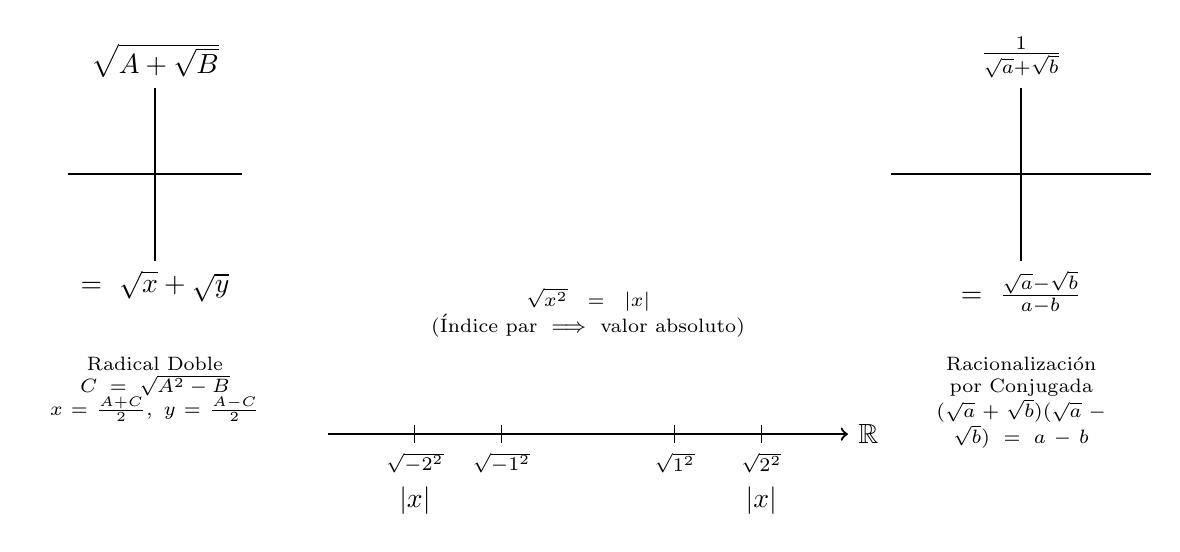
\begin{tikzpicture}[scale=1.1]

  % Radical doble simple
  \begin{scope}[shift={(-5,0)}]
    \draw[thick] (-1,0) -- (1,0);
    \draw[thick] (0,-1) -- (0,1);
    \node[above] at (0, 1) {$\sqrt{A + \sqrt{B}}$};
    \node[below] at (0, -1) {$=\ \sqrt{x} + \sqrt{y}$};
    \node[below, align=center, text width=3cm, font=\scriptsize] at (0, -2) {
      Radical Doble\\
      $C = \sqrt{A^2 - B}$\\
      $x = \frac{A+C}{2},\ y = \frac{A-C}{2}$
    };
  \end{scope}

  % Racionalización por conjugada
  \begin{scope}[shift={(5,0)}]
    \draw[thick] (-1.5, 0) -- (1.5, 0);
    \draw[thick] (0, -1) -- (0, 1);
    \node[above] at (0, 1) {$\frac{1}{\sqrt{a} + \sqrt{b}}$};
    \node[below] at (0, -1) {$=\ \frac{\sqrt{a} - \sqrt{b}}{a - b}$};
    \node[below, align=center, text width=3cm, font=\scriptsize] at (0, -2) {
      Racionalización\\
      por Conjugada\\
      $(\sqrt{a}+\sqrt{b})(\sqrt{a}-\sqrt{b}) = a-b$
    };
  \end{scope}

  % Raíces en la recta real
  \begin{scope}[shift={(0,-3)}]
    \draw[->, thick] (-3, 0) -- (3, 0) node[right] {$\mathbb{R}$};
    \foreach \x in {-2,-1,1,2} {
      \draw (\x,0.1) -- (\x,-0.1) node[below] {\scriptsize $\sqrt{\x^2}$};
    }
    \node[below] at (-2, -0.5) {$|x|$};
    \node[below] at (2, -0.5) {$|x|$};
    \node[above, align=center, text width=4cm, font=\scriptsize] at (0, 1) {
      $\sqrt{x^2} = |x|$\\
      (Índice par $\implies$ valor absoluto)
    };
  \end{scope}

\end{tikzpicture}

\end{document}
